Il gruppo \Gruppo{} ha deciso di pianificare il lavoro seguendo il modello di sviluppo incrementale.

\subsection{Descrizione}
La scelta di un modello di sviluppo porta dei vincoli sulla pianificazione e sulla gestione del progetto.
L’obiettivo del gruppo è di abbinare qualità al modello scelto, in modo da ottenere conformità con
gli obiettivi del modello nel progetto e maturità nei processi.
Il gruppo ha optato di scegliere il modello incrementale per il \glo{ciclo di vita} del software per i seguenti
motivi:
\begin{itemize}
    \item Può produrre valore ad ogni incremento, aiutando a fissare meglio i requisiti per gli incrementi
    successivi;
    \item Ogni incremento riduce il rischio di fallimento;
    \item Le funzionalità principali e/o critiche sono sviluppate nei primi incrementi che diventano via via più stabili.
\end{itemize}



Nel modello incrementale i requisiti vengono classificati in base alla loro importanza strategica. In
questo modo quelli più importanti vengono trattati prima. Questo ne aumenta la chiarezza e la
facilità di soddisfazione. I requisiti meno importanti invece vengono soddisfatti dopo quelli più
importanti venendo cosi inseriti in un sistema già stabilizzato.
Il metodo di lavoro sarà quindi questo:
\begin{itemize}
    \item In ogni fase di lavoro vengono prefissati degli incrementi che devono essere prodotti entro un
    scadenza decisa dal gruppo;
    \item Il lavoro viene diviso tra i membri del gruppo;
    \item Al termine del periodo prefissato una riunione servirà per analizzare il lavoro svolto da ogni
    membro, riscontrare problemi e difficoltà;
    \item Sarà compito dei verificatori controllare il lavoro svolto dagli altri membri del gruppo e sollevare
    eventuali incongruenze o errori;
    \item Alla fine di questa \glo{verifica} seguirà una nuova discussione di gruppo per stabilire se gli obiettivi
    dell’incremento sono stati soddisfatti.
\end{itemize}






\begin{figure}[h!]
    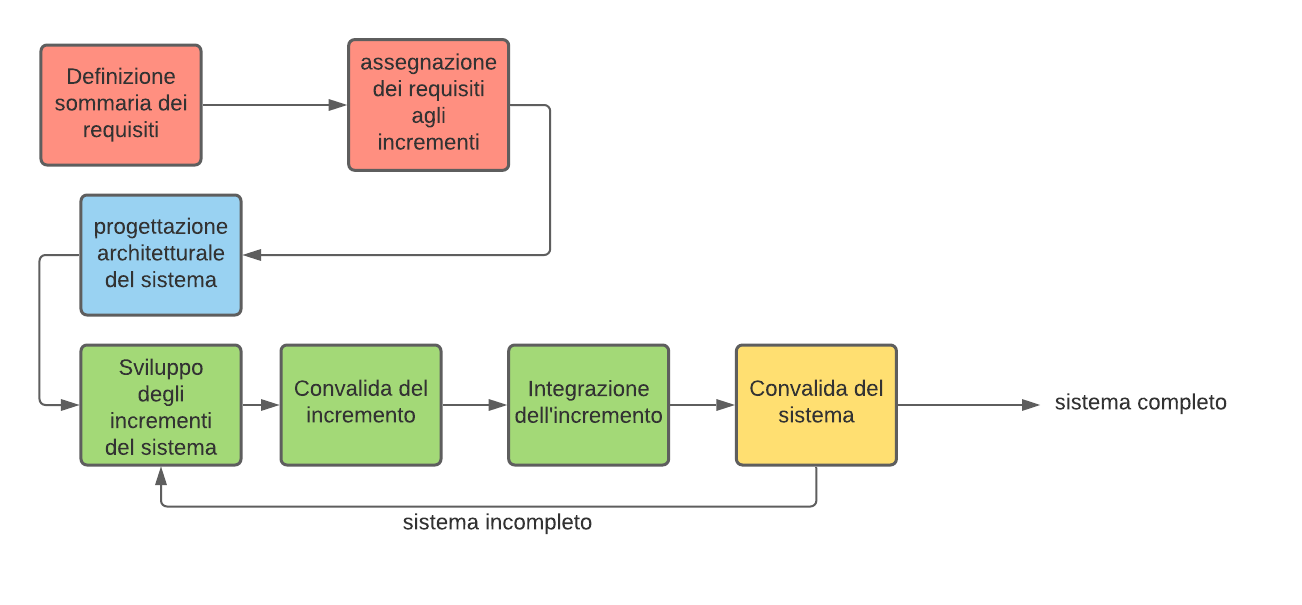
\includegraphics[width=1\textwidth]{./src/ModelloSviluppo/src/img/diagramma modello di sviluppo.png}
    \caption{Modello Incrementale tratto dal libro di Ian Somerville:Software Engineering ottava edizione}
\end{figure}